\chapter{Experiments}\label{chapter:experiments}
in which we try to replicate results from \cite{belkina19}. 

\section{Effect of Varying Perplexity Values}
\begin{figure}[ht]
    \centering 
    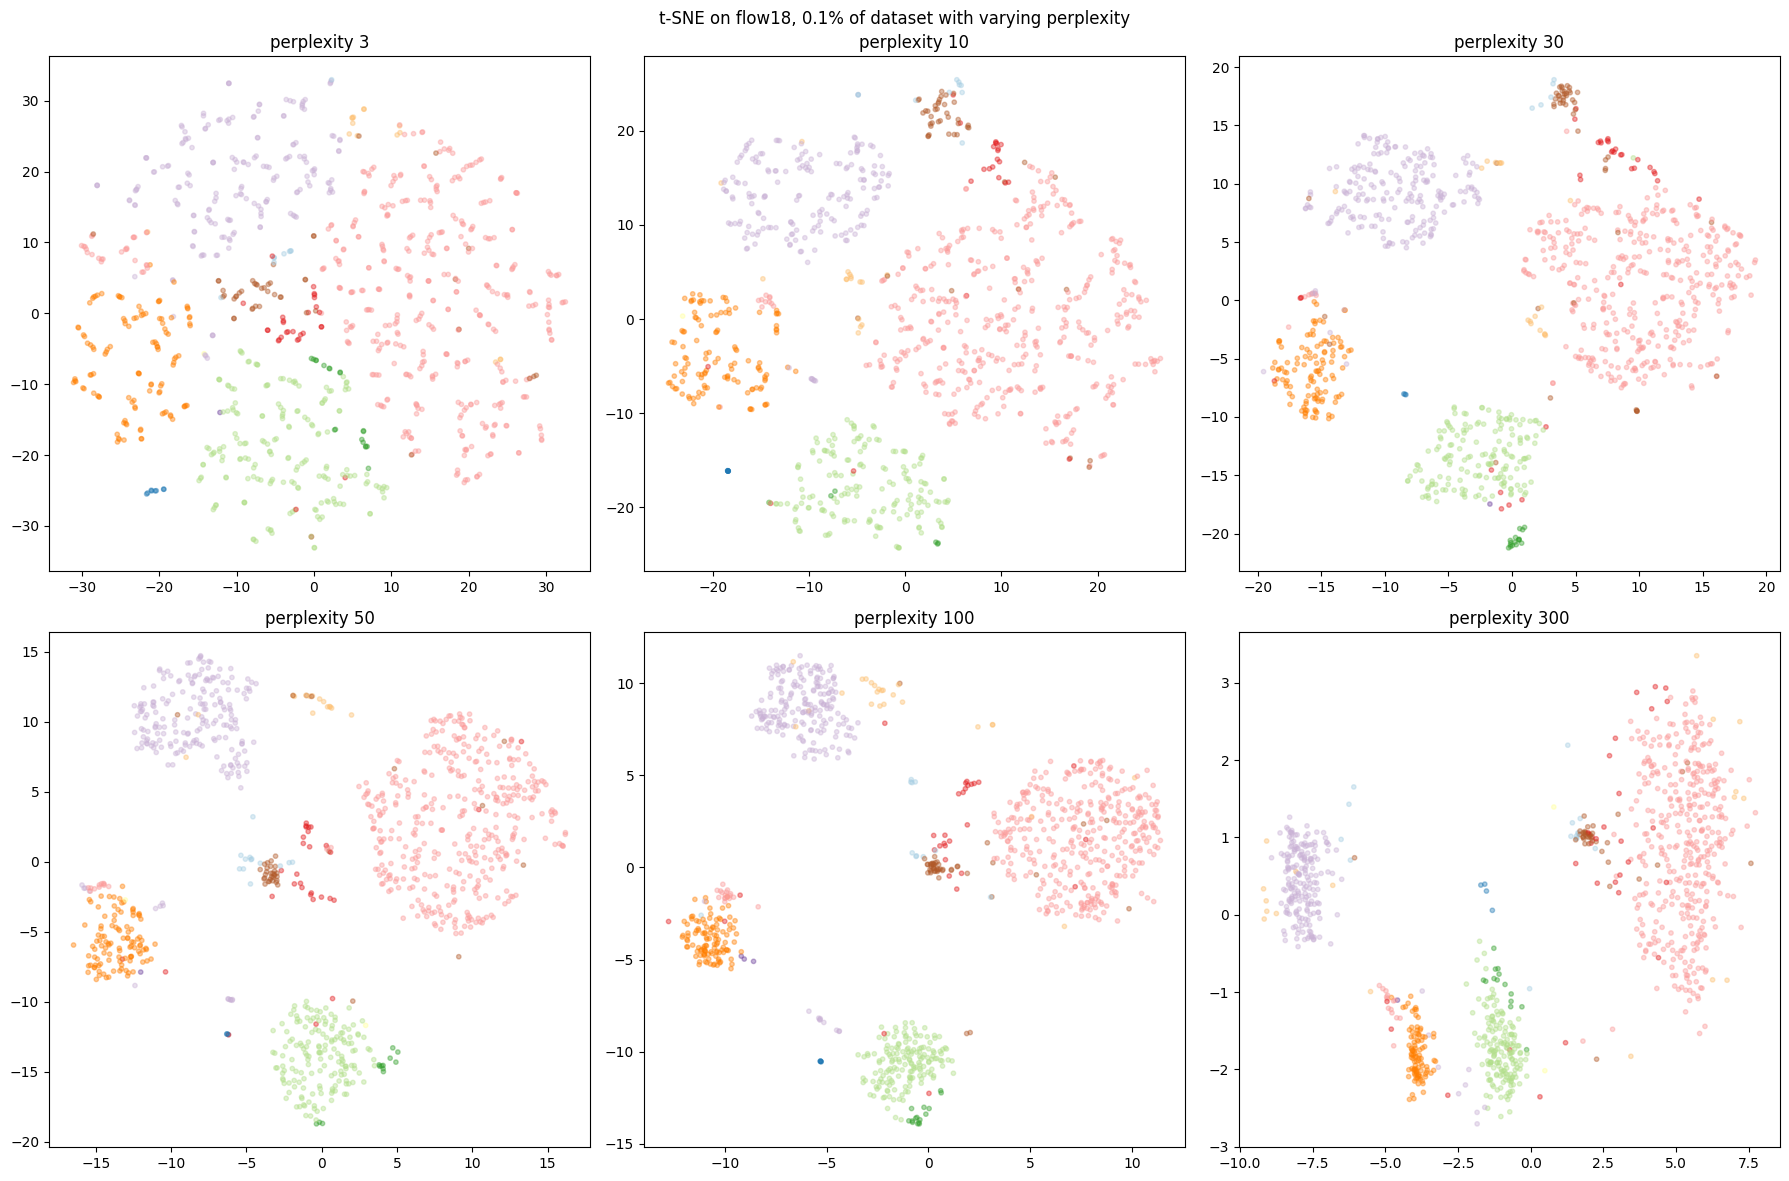
\includegraphics[width=\linewidth]{figures/perp_flow_001.png}
    \caption{Different perplexity values on 0.1 percent the flow18 dataset}
    \label{fig:perp001}
\end{figure}

\begin{figure}[ht]
    \centering 
    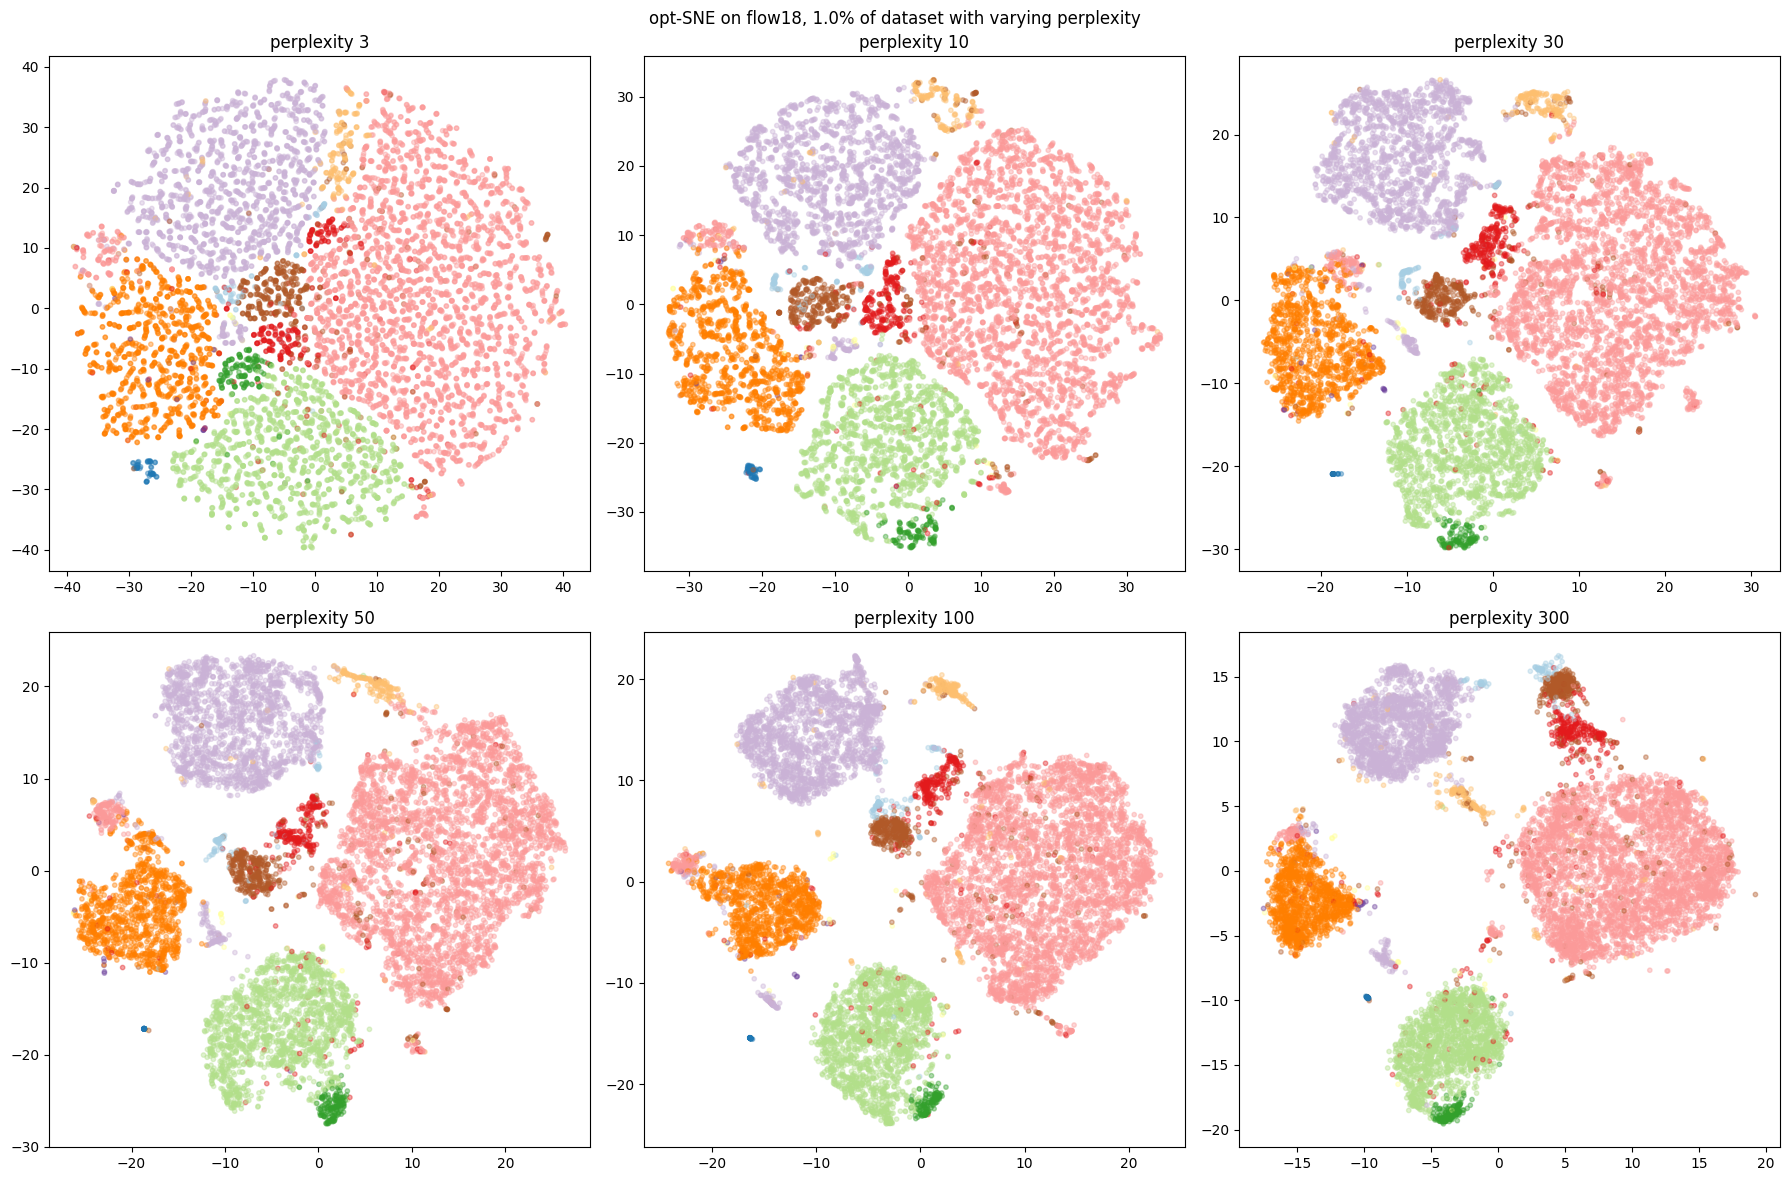
\includegraphics[width=\linewidth]{figures/perp_flow_01.png}
    \caption{Different perplexity values on 1 percent the flow18 dataset}
    \label{fig:perp01}
\end{figure}

\begin{figure}[ht]
    \centering 
    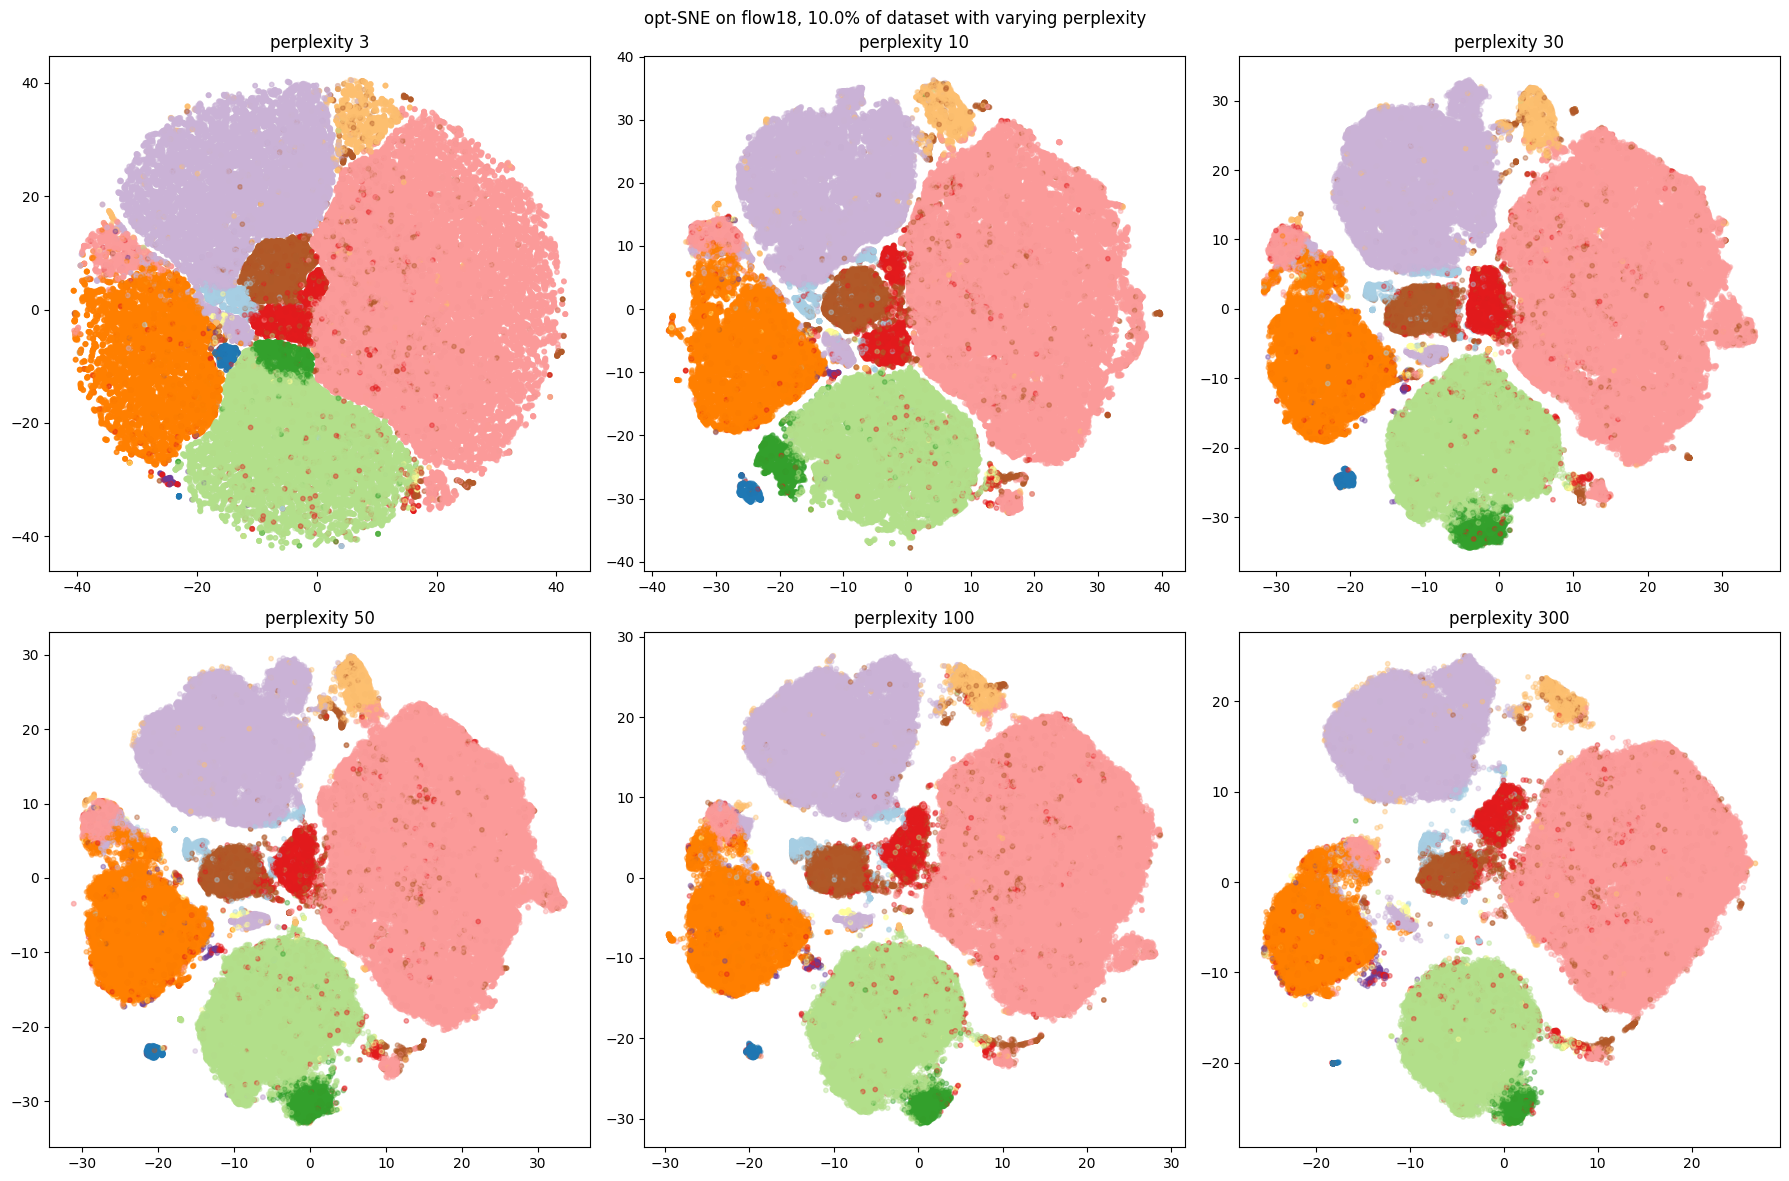
\includegraphics[width=\linewidth]{figures/perp_flow_1.png}
    \caption{Different perplexity values on 10 percent the flow18 dataset}
    \label{fig:perp1}
\end{figure}

\begin{figure}[ht]
    \centering 
    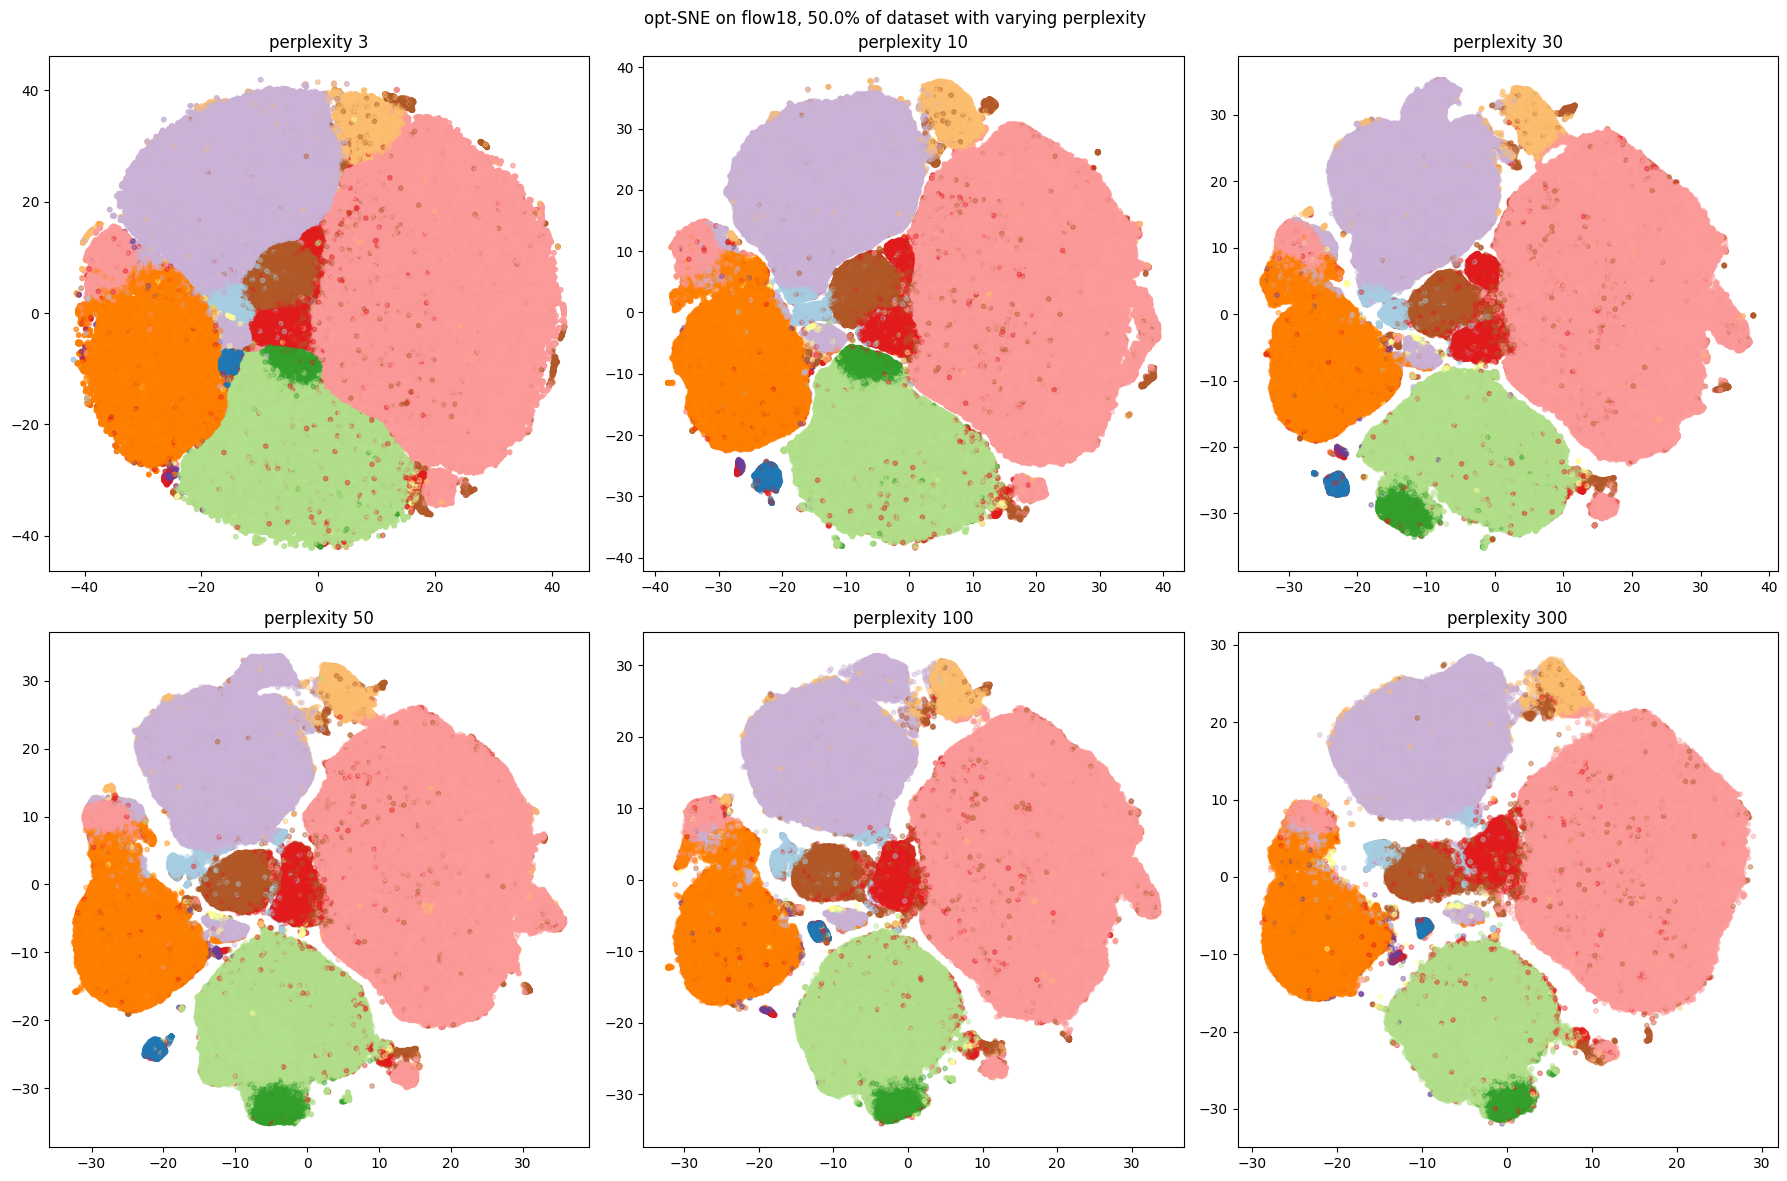
\includegraphics[width=\linewidth]{figures/perp_flow_5.png}
    \caption{Different perplexity values on 50 percent the flow18 dataset}
    \label{fig:perp5}
\end{figure}